%%%%%%%%%%%%%%%%%%%%%%%%%%%%%%%%%%%%%%%%%
% Beamer Presentation
% LaTeX Template
% Version 1.0 (10/11/12)
%
% This template has been downloaded from:
% http://www.LaTeXTemplates.com
%
% License:
% CC BY-NC-SA 3.0 (http://creativecommons.org/licenses/by-nc-sa/3.0/)
%
%%%%%%%%%%%%%%%%%%%%%%%%%%%%%%%%%%%%%%%%%

%----------------------------------------------------------------------------------------
%	PACKAGES AND THEMES
%----------------------------------------------------------------------------------------

\documentclass{beamer}

\mode<presentation> {

% The Beamer class comes with a number of default slide themes
% which change the colors and layouts of slides. Below this is a list
% of all the themes, uncomment each in turn to see what they look like.

%\usetheme{default}
%\usetheme{AnnArbor}
%\usetheme{Antibes}
%\usetheme{Bergen}
%\usetheme{Berkeley}
%\usetheme{Berlin}
%\usetheme{Boadilla}
%\usetheme{CambridgeUS}
%\usetheme{Copenhagen}
%\usetheme{Darmstadt}
%\usetheme{Dresden}
%\usetheme{Frankfurt}
%\usetheme{Goettingen}
%\usetheme{Hannover}
\usetheme{Ilmenau} % best so far
%\usetheme{JuanLesPins}
%\usetheme{Luebeck}
%\usetheme{Madrid}
%\usetheme{Malmoe}
%\usetheme{Marburg}
%\usetheme{Montpellier}
%\usetheme{PaloAlto}
%\usetheme{Pittsburgh}
%\usetheme{Rochester}
%\usetheme{Singapore}
%\usetheme{Szeged}
%\usetheme{Warsaw}

% As well as themes, the Beamer class has a number of color themes
% for any slide theme. Uncomment each of these in turn to see how it
% changes the colors of your current slide theme.

%\usecolortheme{albatross}
%\usecolortheme{beaver}
%\usecolortheme{beetle}
%\usecolortheme{crane}
%\usecolortheme{dolphin}
%\usecolortheme{dove}
%\usecolortheme{fly}
\usecolortheme{lily}
%\usecolortheme{orchid}
%\usecolortheme{rose}
%\usecolortheme{seagull}
%\usecolortheme{seahorse}
%\usecolortheme{whale}
%\usecolortheme{wolverine}

%\setbeamertemplate{footline} % To remove the footer line in all slides uncomment this line
\setbeamertemplate{footline}[page number] % To replace the footer line in all slides with a simple slide count uncomment this line

%\setbeamertemplate{navigation symbols}{} % To remove the navigation symbols from the bottom of all slides uncomment this line
}

\usepackage{graphicx} % Allows including images
\usepackage{booktabs} % Allows the use of \toprule, \midrule and \bottomrule in tables
\usepackage{csquotes}
\usepackage[font=tiny,labelfont=bf]{caption}
\usepackage{url}
\usepackage{qtree}
\usepackage{float}
\usepackage{tikz}
\usetikzlibrary{automata, positioning, arrows}

\graphicspath{{figures/}}
\bibliographystyle{abbrv}

\let\oldquote\quote
\let\endoldquote\endquote
\renewenvironment{quote}[2][]
{\if\relax\detokenize{#1}\relax
	\def\quoteauthor{#2}%
	\else
	\def\quoteauthor{#2~---~#1}%
	\fi
	\oldquote}
{\par\nobreak\smallskip\hfill(\quoteauthor)%
	\endoldquote\addvspace{\bigskipamount}}


%----------------------------------------------------------------------------------------
%	TITLE PAGE
%----------------------------------------------------------------------------------------

\title[Formalization]{Peter Naur's contribution to formal notations and beyond} % The short title appears at the bottom of every slide, the full title is only on the title page

\author{Viktor Gsteiger} % Your name
\institute[unibas] % Your institution as it will appear on the bottom of every slide, may be shorthand to save space
{
University of Basel \\ % Your institution for the title page
\medskip
\textit{Seminar Turing Award Winners and Their Contributions} \\
\textit{v.gsteiger@unibas.ch} % Your email address
}
\date{November 26, 2020} % Date, can be changed to a custom date

\begin{document}

\begin{frame}
\titlepage % Print the title page as the first slide
\end{frame}

\begin{frame}
	\frametitle{Peter Naur}
	\begin{figure}
		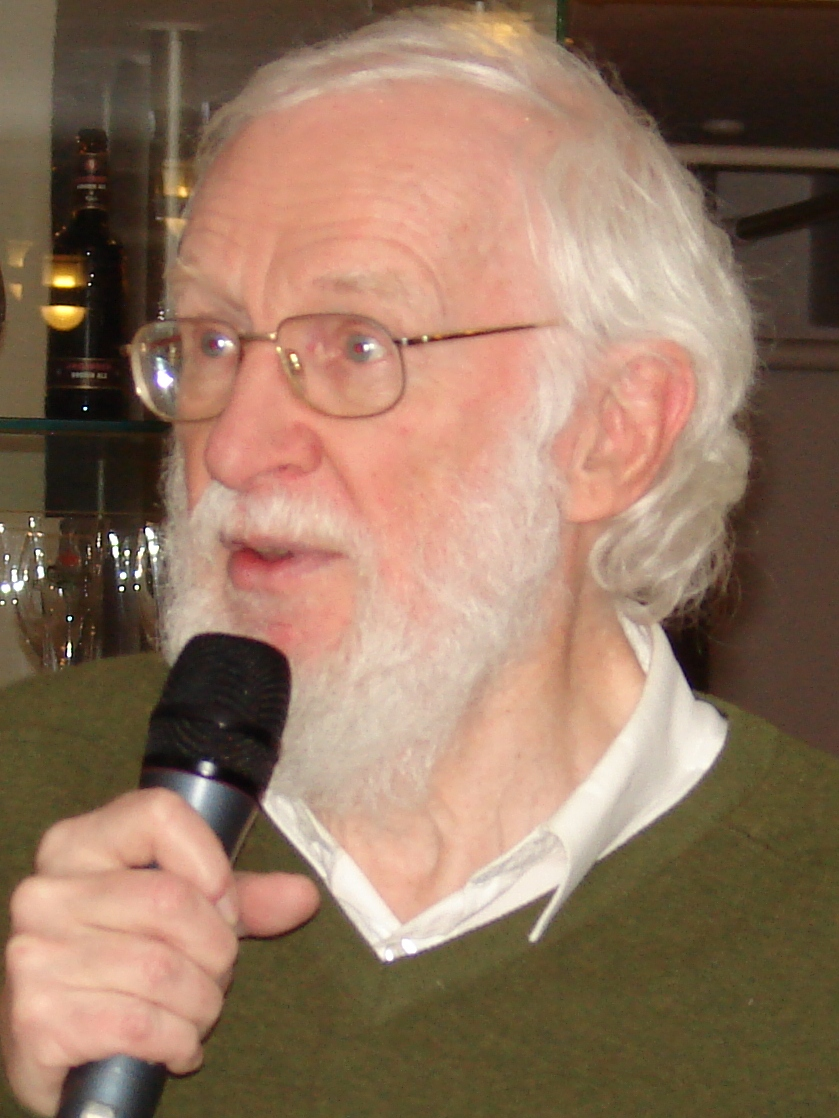
\includegraphics[height=\dimexpr
		\textheight-3\baselineskip-\parskip-.2em-
		\abovecaptionskip-\belowcaptionskip\relax]{Peternaur}
		\caption{\cite{naur}}
		\label{fig:naur}
	\end{figure}
\end{frame}

\begin{frame}
	\frametitle{Peter Naur's contribution}
	
	\blockquote{For fundamental contributions to programming language design and the definition of Algol 60, to compiler design, and to the art and practice of computer programming.}
\end{frame}

\begin{frame}
	\frametitle{Formal notations in history}
	
	\begin{figure}
		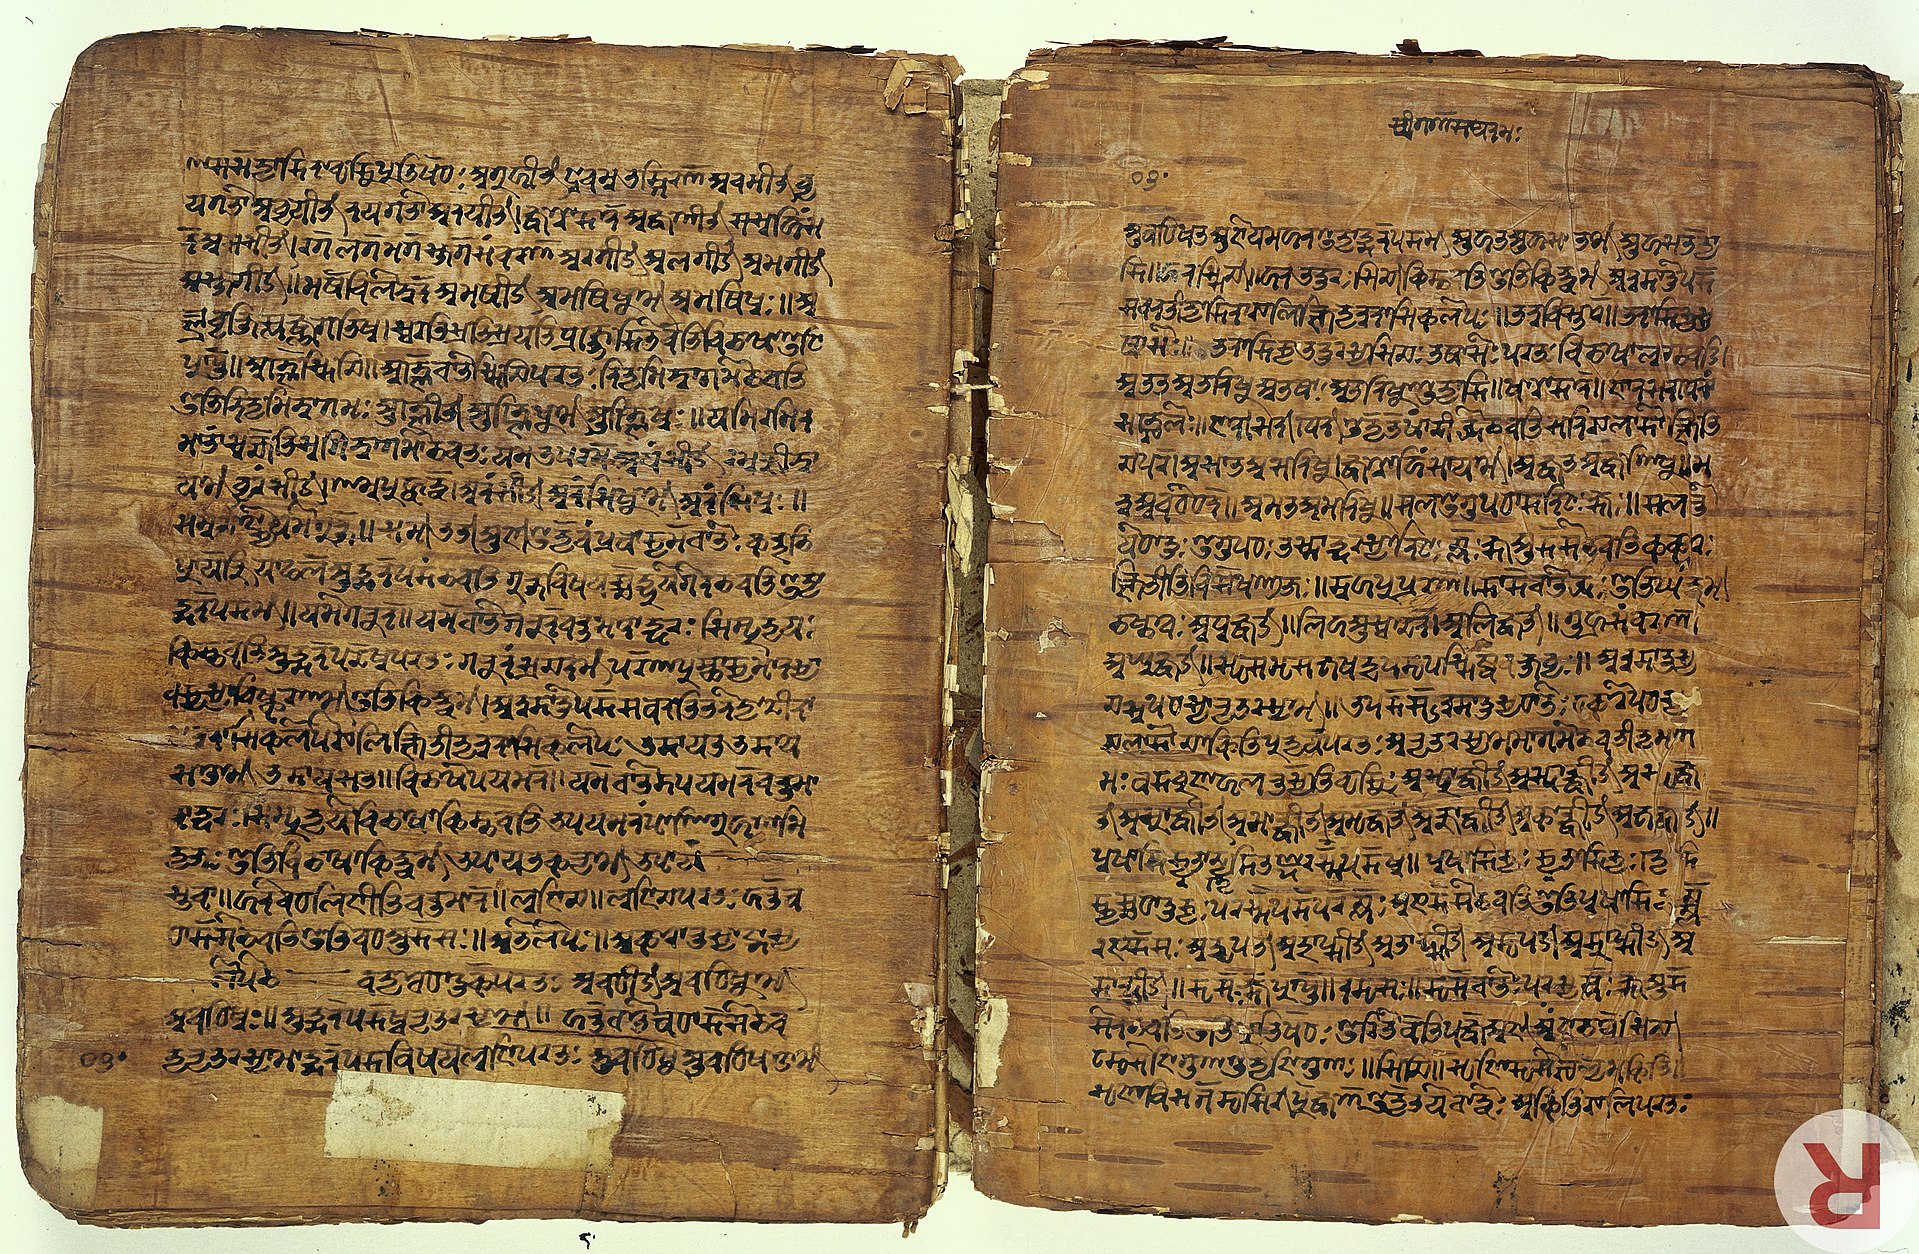
\includegraphics[width=8cm]{1920px-Birch_bark_MS_from_Kashmir_of_the_Rupavatra_Wellcome_L0032691}
		\caption{\cite{birch}}
		\label{fig:bark}
	\end{figure}
\end{frame}

\begin{frame}
	\frametitle{New need for formal notations}
	
	\begin{figure}
		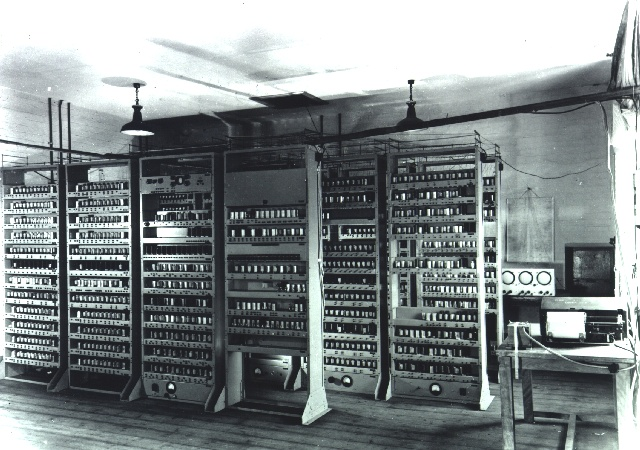
\includegraphics[width=8cm]{EDSAC_(19)}
		\caption{\cite{EDSAC}}
	\end{figure}
\end{frame}

\begin{frame}
\frametitle{Overview} % Table of contents slide, comment this block out to remove it
\tableofcontents % Throughout your presentation, if you choose to use \section{} and \subsection{} commands, these will automatically be printed on this slide as an overview of your presentation
\end{frame}

%----------------------------------------------------------------------------------------
%	PRESENTATION SLIDES
%----------------------------------------------------------------------------------------

%------------------------------------------------
\section{Formal notations} % Sections can be created in order to organize your presentation into discrete blocks, all sections and subsections are automatically printed in the table of contents as an overview of the talk
%------------------------------------------------

\subsection{Phrase structure grammars} % A subsection can be created just before a set of slides with a common theme to further break down your presentation into chunks

\begin{frame}
	\frametitle{Phrase structure definition}
	\begin{equation} \label{eq1}
	\begin{split}
	\sum &: \# Sentence \# \\
	F&: \\ Sentence &\to NP\_VP \\
	VP &\to Verb\_NP \\
	NP &\to \text{the man}, \text{the book} \\
	Verb &\to \text{took}
	\end{split}
	\end{equation}
\end{frame}

\begin{frame}
\frametitle{Phrase structure in tree form}
\begin{equation} \label{eq2}
	\Tree[.Sentence [.NP [ \textit{the man} ]]
			  [.VP [.Verb \textit{took} ]
					[.NP [.\textit{the book} ]]]]
\end{equation}
\end{frame}

%------------------------------------------------

\subsection{Backus Naur form}

\begin{frame}
\frametitle{Backus Naur form}
\begin{equation} \label{eq2}
	\begin{split}
	<sentence> &::=<NP>\text{ }<VP> \\
	<VP> &::=<Verb>\text{ }<NP> \\
	<NP> &::=\text{the man}\text{ }|\text{ }\text{the book} \\
	<Verb> &::=\text{took} \\
\end{split}
\end{equation}
\end{frame}

%------------------------------------------------

\subsection{Programming languages, natural languages and mathematical languages}

\begin{frame}
\frametitle{Comparison of levels of formalization}
\begin{itemize}
	\item Natural languages
	\item Mathematical languages
	\item Programming languages
\end{itemize}
\end{frame}

%------------------------------------------------
\section{Peter Naur's contribution}
%------------------------------------------------

\subsection{Definition of Algol 60}

\begin{frame}
\frametitle{Table}
\begin{table}
\begin{tabular}{l l l}
\toprule
\textbf{Treatments} & \textbf{Response 1} & \textbf{Response 2}\\
\midrule
Treatment 1 & 0.0003262 & 0.562 \\
Treatment 2 & 0.0015681 & 0.910 \\
Treatment 3 & 0.0009271 & 0.296 \\
\bottomrule
\end{tabular}
\caption{Table caption}
\end{table}
\end{frame}

%------------------------------------------------

\subsection{Compiler Design}

\begin{frame}
\frametitle{Theorem}
\begin{theorem}[Mass--energy equivalence]
$E = mc^2$
\end{theorem}
\end{frame}

%------------------------------------------------

\subsection{Art and practice of computer programming}

\begin{frame}[fragile] % Need to use the fragile option when verbatim is used in the slide
\frametitle{Verbatim}
\begin{example}[Theorem Slide Code]
\begin{verbatim}
\begin{frame}
\frametitle{Theorem}
\begin{theorem}[Mass--energy equivalence]
$E = mc^2$
\end{theorem}
\end{frame}\end{verbatim}
\end{example}
\end{frame}

%------------------------------------------------

\begin{frame}
\frametitle{Figure}
Uncomment the code on this slide to include your own image from the same directory as the template .TeX file.
%\begin{figure}
%\includegraphics[width=0.8\linewidth]{test}
%\end{figure}
\end{frame}

%------------------------------------------------

\begin{frame}[fragile] % Need to use the fragile option when verbatim is used in the slide
\frametitle{Citation}
An example of the \verb|\cite| command to cite within the presentation:\\~

This statement requires citation \cite{birch}.
\end{frame}

\section{Computing vs. Human Thinking}

%------------------------------------------------

\begin{frame} % Need to use the fragile option when verbatim is used in the slide
	\frametitle{Computing Versus Human Thinking}
	\begin{itemize}
		\item Description of computers
		\item Description of human thinking
	\end{itemize}
\end{frame}

%------------------------------------------------

\begin{frame}
	\frametitle{Discussion}
	\textbf{Do you think that human thinking will be formally describable?}
\end{frame}

%------------------------------------------------

\section{Conclusion}

\begin{frame}[fragile] % Need to use the fragile option when verbatim is used in the slide
	\frametitle{Importance of formal notation}
	\begin{quote}{Peter Naur}
			For achieving clarity any formal mode of expression should be used, not as a goal in itself, but wherever it appears to be helpful to authors and readers alike.
	\end{quote}
\end{frame}

%------------------------------------------------

%------------------------------------------------

\begin{frame}
	\Huge{\centerline{The End}}
\end{frame}

%----------------------------------------------------------------------------------------
\begin{frame}
	\frametitle{References}
	\footnotesize{
		\bibliography{references}
	}
\end{frame}

\end{document} 